\documentclass{book}
\usepackage[a4paper,top=2.5cm,bottom=2.5cm,left=2.5cm,right=2.5cm]{geometry}
\usepackage{makeidx}
\usepackage{natbib}
\usepackage{graphicx}
\usepackage{multicol}
\usepackage{float}
\usepackage{listings}
\usepackage{color}
\usepackage{ifthen}
\usepackage[table]{xcolor}
\usepackage{textcomp}
\usepackage{alltt}
\usepackage{ifpdf}
\ifpdf
\usepackage[pdftex,
            pagebackref=true,
            colorlinks=true,
            linkcolor=blue,
            unicode
           ]{hyperref}
\else
\usepackage[ps2pdf,
            pagebackref=true,
            colorlinks=true,
            linkcolor=blue,
            unicode
           ]{hyperref}
\usepackage{pspicture}
\fi
\usepackage[utf8]{inputenc}
\usepackage{mathptmx}
\usepackage[scaled=.90]{helvet}
\usepackage{courier}
\usepackage{sectsty}
\usepackage{amssymb}
\usepackage[titles]{tocloft}
\usepackage{doxygen}
\lstset{language=C++,inputencoding=utf8,basicstyle=\footnotesize,breaklines=true,breakatwhitespace=true,tabsize=4,numbers=left }
\makeindex
\setcounter{tocdepth}{3}
\renewcommand{\footrulewidth}{0.4pt}
\renewcommand{\familydefault}{\sfdefault}
\hfuzz=15pt
\setlength{\emergencystretch}{15pt}
\hbadness=750
\tolerance=750
\begin{document}
\hypersetup{pageanchor=false,citecolor=blue}
\begin{titlepage}
\vspace*{7cm}
\begin{center}
{\Large My Project }\\
\vspace*{1cm}
{\large Generated by Doxygen 1.8.2}\\
\vspace*{0.5cm}
{\small Tue May 17 2016 17:00:39}\\
\end{center}
\end{titlepage}
\clearemptydoublepage
\pagenumbering{roman}
\tableofcontents
\clearemptydoublepage
\pagenumbering{arabic}
\hypersetup{pageanchor=true,citecolor=blue}
\chapter{Doxygen工程演示}
\label{index}\hypertarget{index}{}\hypertarget{index_介绍}{}\section{介绍}\label{index_介绍}
本工程总共只有4个文件 \hyperlink{base_8h}{base.\-h} \hyperlink{dbbase_8h}{dbbase.\-h} \hyperlink{dbbase_8cpp}{dbbase.\-cpp} \hyperlink{sql_8cpp}{sql.\-cpp} \par
 
\chapter{Data Structure Index}
\section{Data Structures}
Here are the data structures with brief descriptions\-:\begin{DoxyCompactList}
\item\contentsline{section}{\hyperlink{structAppRtuInfo}{App\-Rtu\-Info} }{\pageref{structAppRtuInfo}}{}
\item\contentsline{section}{\hyperlink{structDBTypeInfo}{D\-B\-Type\-Info} }{\pageref{structDBTypeInfo}}{}
\item\contentsline{section}{\hyperlink{structDetectorBind}{Detector\-Bind} }{\pageref{structDetectorBind}}{}
\item\contentsline{section}{\hyperlink{structDetectorInfo}{Detector\-Info} }{\pageref{structDetectorInfo}}{}
\item\contentsline{section}{\hyperlink{structDetectorRtu}{Detector\-Rtu} }{\pageref{structDetectorRtu}}{}
\item\contentsline{section}{\hyperlink{structExNativeRtu}{Ex\-Native\-Rtu} }{\pageref{structExNativeRtu}}{}
\item\contentsline{section}{\hyperlink{structHostMan}{Host\-Man} }{\pageref{structHostMan}}{}
\item\contentsline{section}{\hyperlink{structHostRegInfo}{Host\-Reg\-Info} }{\pageref{structHostRegInfo}}{}
\item\contentsline{section}{\hyperlink{structMysqlConInfo}{Mysql\-Con\-Info} }{\pageref{structMysqlConInfo}}{}
\item\contentsline{section}{\hyperlink{structNativeRtuInfo}{Native\-Rtu\-Info} }{\pageref{structNativeRtuInfo}}{}
\item\contentsline{section}{\hyperlink{structRelayInfo}{Relay\-Info} }{\pageref{structRelayInfo}}{}
\item\contentsline{section}{\hyperlink{structRtuBind}{Rtu\-Bind} }{\pageref{structRtuBind}}{}
\item\contentsline{section}{\hyperlink{structRtuRegInfo}{Rtu\-Reg\-Info} }{\pageref{structRtuRegInfo}}{}
\item\contentsline{section}{\hyperlink{structRtuRemoveInfo}{Rtu\-Remove\-Info} }{\pageref{structRtuRemoveInfo}}{}
\item\contentsline{section}{\hyperlink{structRtuUpdate}{Rtu\-Update} }{\pageref{structRtuUpdate}}{}
\item\contentsline{section}{\hyperlink{structSafetyPwdInfo}{Safety\-Pwd\-Info} }{\pageref{structSafetyPwdInfo}}{}
\item\contentsline{section}{\hyperlink{structSafetyRtu}{Safety\-Rtu} }{\pageref{structSafetyRtu}}{}
\item\contentsline{section}{\hyperlink{structSceneBind}{Scene\-Bind} }{\pageref{structSceneBind}}{}
\item\contentsline{section}{\hyperlink{structSceneInfo}{Scene\-Info} }{\pageref{structSceneInfo}}{}
\item\contentsline{section}{\hyperlink{structSceneRtu}{Scene\-Rtu} }{\pageref{structSceneRtu}}{}
\item\contentsline{section}{\hyperlink{structTaskInfo}{Task\-Info} }{\pageref{structTaskInfo}}{}
\end{DoxyCompactList}

\chapter{File Index}
\section{File List}
Here is a list of all files with brief descriptions\-:\begin{DoxyCompactList}
\item\contentsline{section}{\hyperlink{AddrDefine_8h}{Addr\-Define.\-h} \\*地址定义 }{\pageref{AddrDefine_8h}}{}
\item\contentsline{section}{\hyperlink{CommonType_8h}{Common\-Type.\-h} \\*常见类型定义 }{\pageref{CommonType_8h}}{}
\item\contentsline{section}{\hyperlink{DoxygenFile_8c}{Doxygen\-File.\-c} }{\pageref{DoxygenFile_8c}}{}
\item\contentsline{section}{\hyperlink{DoxygenFile_8h}{Doxygen\-File.\-h} \\*中间层,用于处理数据 }{\pageref{DoxygenFile_8h}}{}
\item\contentsline{section}{\hyperlink{HandleFile_8c}{Handle\-File.\-c} }{\pageref{HandleFile_8c}}{}
\item\contentsline{section}{\hyperlink{HandleFile_8h}{Handle\-File.\-h} }{\pageref{HandleFile_8h}}{}
\item\contentsline{section}{\hyperlink{main_8c}{main.\-c} }{\pageref{main_8c}}{}
\item\contentsline{section}{\hyperlink{RetCode_8h}{Ret\-Code.\-h} \\*错误码返回值 }{\pageref{RetCode_8h}}{}
\end{DoxyCompactList}

\chapter{Data Structure Documentation}
\hypertarget{structCoordinator}{\section{Coordinator Struct Reference}
\label{structCoordinator}\index{Coordinator@{Coordinator}}
}


{\ttfamily \#include $<$Common\-Type.\-h$>$}

\subsection*{Data Fields}
\begin{DoxyCompactItemize}
\item 
int \hyperlink{structCoordinator_a457b1fc480109793f6bdfc23417b54c1}{x}
\begin{DoxyCompactList}\small\item\em 横坐标 \end{DoxyCompactList}\item 
int \hyperlink{structCoordinator_a342fba35825c82ec69bc300823bd3579}{y}
\begin{DoxyCompactList}\small\item\em 纵坐标 \end{DoxyCompactList}\end{DoxyCompactItemize}


\subsection{Detailed Description}
坐标系类型 

\subsection{Field Documentation}
\hypertarget{structCoordinator_a457b1fc480109793f6bdfc23417b54c1}{\index{Coordinator@{Coordinator}!x@{x}}
\index{x@{x}!Coordinator@{Coordinator}}
\subsubsection[{x}]{\setlength{\rightskip}{0pt plus 5cm}int Coordinator\-::x}}\label{structCoordinator_a457b1fc480109793f6bdfc23417b54c1}


横坐标 

\hypertarget{structCoordinator_a342fba35825c82ec69bc300823bd3579}{\index{Coordinator@{Coordinator}!y@{y}}
\index{y@{y}!Coordinator@{Coordinator}}
\subsubsection[{y}]{\setlength{\rightskip}{0pt plus 5cm}int Coordinator\-::y}}\label{structCoordinator_a342fba35825c82ec69bc300823bd3579}


纵坐标 



The documentation for this struct was generated from the following file\-:\begin{DoxyCompactItemize}
\item 
\hyperlink{CommonType_8h}{Common\-Type.\-h}\end{DoxyCompactItemize}

\chapter{File Documentation}
\hypertarget{AddrDefine_8h}{\section{Addr\-Define.\-h File Reference}
\label{AddrDefine_8h}\index{Addr\-Define.\-h@{Addr\-Define.\-h}}
}


地址定义  


This graph shows which files directly or indirectly include this file\-:\nopagebreak
\begin{figure}[H]
\begin{center}
\leavevmode
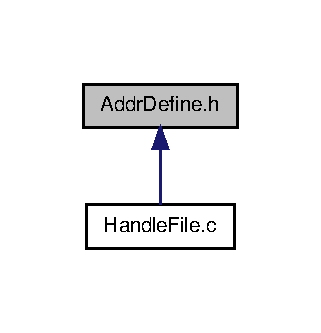
\includegraphics[width=154pt]{AddrDefine_8h__dep__incl}
\end{center}
\end{figure}
\subsection*{Macros}
\begin{DoxyCompactItemize}
\item 
\#define \hyperlink{AddrDefine_8h_a1941f21ee3c59a665a0cff59fc15cbdf}{A\-D\-D\-R\-\_\-\-F\-I\-L\-E\-\_\-\-S\-T\-A\-R\-T}~0x00000000
\begin{DoxyCompactList}\small\item\em 文件起始地址 \end{DoxyCompactList}\item 
\#define \hyperlink{AddrDefine_8h_abc9315b4eafb6b138ba89e6695ece80b}{A\-D\-D\-R\-\_\-\-D\-I\-R\-\_\-\-S\-T\-A\-R\-T}~0x00000001
\begin{DoxyCompactList}\small\item\em 目录起始地址 \end{DoxyCompactList}\end{DoxyCompactItemize}


\subsection{Detailed Description}
地址定义 

\subsection{Macro Definition Documentation}
\hypertarget{AddrDefine_8h_abc9315b4eafb6b138ba89e6695ece80b}{\index{Addr\-Define.\-h@{Addr\-Define.\-h}!A\-D\-D\-R\-\_\-\-D\-I\-R\-\_\-\-S\-T\-A\-R\-T@{A\-D\-D\-R\-\_\-\-D\-I\-R\-\_\-\-S\-T\-A\-R\-T}}
\index{A\-D\-D\-R\-\_\-\-D\-I\-R\-\_\-\-S\-T\-A\-R\-T@{A\-D\-D\-R\-\_\-\-D\-I\-R\-\_\-\-S\-T\-A\-R\-T}!AddrDefine.h@{Addr\-Define.\-h}}
\subsubsection[{A\-D\-D\-R\-\_\-\-D\-I\-R\-\_\-\-S\-T\-A\-R\-T}]{\setlength{\rightskip}{0pt plus 5cm}\#define A\-D\-D\-R\-\_\-\-D\-I\-R\-\_\-\-S\-T\-A\-R\-T~0x00000001}}\label{AddrDefine_8h_abc9315b4eafb6b138ba89e6695ece80b}


目录起始地址 

\hypertarget{AddrDefine_8h_a1941f21ee3c59a665a0cff59fc15cbdf}{\index{Addr\-Define.\-h@{Addr\-Define.\-h}!A\-D\-D\-R\-\_\-\-F\-I\-L\-E\-\_\-\-S\-T\-A\-R\-T@{A\-D\-D\-R\-\_\-\-F\-I\-L\-E\-\_\-\-S\-T\-A\-R\-T}}
\index{A\-D\-D\-R\-\_\-\-F\-I\-L\-E\-\_\-\-S\-T\-A\-R\-T@{A\-D\-D\-R\-\_\-\-F\-I\-L\-E\-\_\-\-S\-T\-A\-R\-T}!AddrDefine.h@{Addr\-Define.\-h}}
\subsubsection[{A\-D\-D\-R\-\_\-\-F\-I\-L\-E\-\_\-\-S\-T\-A\-R\-T}]{\setlength{\rightskip}{0pt plus 5cm}\#define A\-D\-D\-R\-\_\-\-F\-I\-L\-E\-\_\-\-S\-T\-A\-R\-T~0x00000000}}\label{AddrDefine_8h_a1941f21ee3c59a665a0cff59fc15cbdf}


文件起始地址 

地址定义 
\hypertarget{CommonType_8h}{\section{Common\-Type.\-h File Reference}
\label{CommonType_8h}\index{Common\-Type.\-h@{Common\-Type.\-h}}
}


常见类型定义  


This graph shows which files directly or indirectly include this file\-:\nopagebreak
\begin{figure}[H]
\begin{center}
\leavevmode
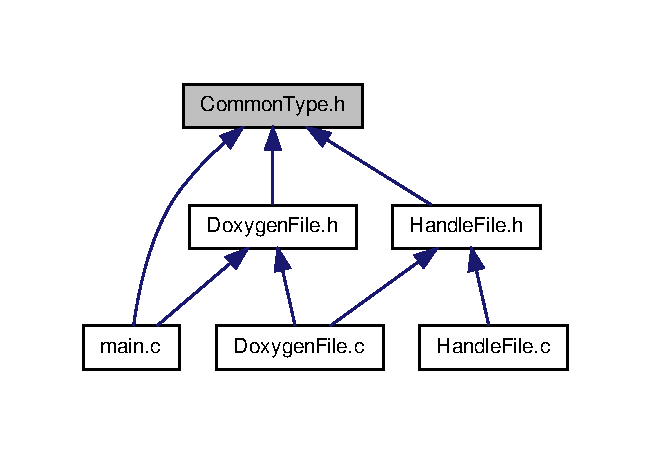
\includegraphics[width=312pt]{CommonType_8h__dep__incl}
\end{center}
\end{figure}
\subsection*{Data Structures}
\begin{DoxyCompactItemize}
\item 
struct \hyperlink{structCoordinator}{Coordinator}
\end{DoxyCompactItemize}
\subsection*{Macros}
\begin{DoxyCompactItemize}
\item 
\#define \hyperlink{CommonType_8h_a070d2ce7b6bb7e5c05602aa8c308d0c4}{N\-U\-L\-L}~0
\end{DoxyCompactItemize}
\subsection*{Typedefs}
\begin{DoxyCompactItemize}
\item 
typedef unsigned int \hyperlink{CommonType_8h_a36cb3b01d81ffd844bbbfb54003e06ec}{U\-I\-N\-T}
\item 
typedef unsigned char \hyperlink{CommonType_8h_a4ae1dab0fb4b072a66584546209e7d58}{B\-Y\-T\-E}
\item 
typedef unsigned short \hyperlink{CommonType_8h_a197942eefa7db30960ae396d68339b97}{W\-O\-R\-D}
\end{DoxyCompactItemize}
\subsection*{Enumerations}
\begin{DoxyCompactItemize}
\item 
enum \hyperlink{CommonType_8h_af90824509586333cf45ce757d2711ce3}{C\-O\-L\-O\-R} \{ \hyperlink{CommonType_8h_af90824509586333cf45ce757d2711ce3af80f9a890089d211842d59625e561f88}{R\-E\-D} =0, 
\hyperlink{CommonType_8h_af90824509586333cf45ce757d2711ce3aa60bd322f93178d68184e30e162571ca}{G\-R\-E\-E\-N} =1, 
\hyperlink{CommonType_8h_af90824509586333cf45ce757d2711ce3ae735a848bf82163a19236ead1c3ef2d2}{Y\-E\-L\-L\-O\-W} =2
 \}
\begin{DoxyCompactList}\small\item\em 枚举类型 \end{DoxyCompactList}\end{DoxyCompactItemize}


\subsection{Detailed Description}
常见类型定义 \begin{DoxyAuthor}{Author}
Vincent 
\end{DoxyAuthor}
\begin{DoxyDate}{Date}
2015-\/5-\/24 
\end{DoxyDate}
\begin{DoxyVersion}{Version}
A001 
\end{DoxyVersion}
\begin{DoxyCopyright}{Copyright}
Vincent 
\end{DoxyCopyright}


\subsection{Macro Definition Documentation}
\hypertarget{CommonType_8h_a070d2ce7b6bb7e5c05602aa8c308d0c4}{\index{Common\-Type.\-h@{Common\-Type.\-h}!N\-U\-L\-L@{N\-U\-L\-L}}
\index{N\-U\-L\-L@{N\-U\-L\-L}!CommonType.h@{Common\-Type.\-h}}
\subsubsection[{N\-U\-L\-L}]{\setlength{\rightskip}{0pt plus 5cm}\#define N\-U\-L\-L~0}}\label{CommonType_8h_a070d2ce7b6bb7e5c05602aa8c308d0c4}
空的宏定义 

Referenced by Handle\-Data(), and main().



\subsection{Typedef Documentation}
\hypertarget{CommonType_8h_a4ae1dab0fb4b072a66584546209e7d58}{\index{Common\-Type.\-h@{Common\-Type.\-h}!B\-Y\-T\-E@{B\-Y\-T\-E}}
\index{B\-Y\-T\-E@{B\-Y\-T\-E}!CommonType.h@{Common\-Type.\-h}}
\subsubsection[{B\-Y\-T\-E}]{\setlength{\rightskip}{0pt plus 5cm}typedef unsigned char {\bf B\-Y\-T\-E}}}\label{CommonType_8h_a4ae1dab0fb4b072a66584546209e7d58}
1字节字符类型 \hypertarget{CommonType_8h_a36cb3b01d81ffd844bbbfb54003e06ec}{\index{Common\-Type.\-h@{Common\-Type.\-h}!U\-I\-N\-T@{U\-I\-N\-T}}
\index{U\-I\-N\-T@{U\-I\-N\-T}!CommonType.h@{Common\-Type.\-h}}
\subsubsection[{U\-I\-N\-T}]{\setlength{\rightskip}{0pt plus 5cm}typedef unsigned int {\bf U\-I\-N\-T}}}\label{CommonType_8h_a36cb3b01d81ffd844bbbfb54003e06ec}
4字节字符类型 \hypertarget{CommonType_8h_a197942eefa7db30960ae396d68339b97}{\index{Common\-Type.\-h@{Common\-Type.\-h}!W\-O\-R\-D@{W\-O\-R\-D}}
\index{W\-O\-R\-D@{W\-O\-R\-D}!CommonType.h@{Common\-Type.\-h}}
\subsubsection[{W\-O\-R\-D}]{\setlength{\rightskip}{0pt plus 5cm}typedef unsigned short {\bf W\-O\-R\-D}}}\label{CommonType_8h_a197942eefa7db30960ae396d68339b97}
2字节字符类型 

\subsection{Enumeration Type Documentation}
\hypertarget{CommonType_8h_af90824509586333cf45ce757d2711ce3}{\index{Common\-Type.\-h@{Common\-Type.\-h}!C\-O\-L\-O\-R@{C\-O\-L\-O\-R}}
\index{C\-O\-L\-O\-R@{C\-O\-L\-O\-R}!CommonType.h@{Common\-Type.\-h}}
\subsubsection[{C\-O\-L\-O\-R}]{\setlength{\rightskip}{0pt plus 5cm}enum {\bf C\-O\-L\-O\-R}}}\label{CommonType_8h_af90824509586333cf45ce757d2711ce3}


枚举类型 

\begin{Desc}
\item[Enumerator\-: ]\par
\begin{description}
\index{R\-E\-D@{R\-E\-D}!Common\-Type.\-h@{Common\-Type.\-h}}\index{Common\-Type.\-h@{Common\-Type.\-h}!R\-E\-D@{R\-E\-D}}\item[{\em 
\hypertarget{CommonType_8h_af90824509586333cf45ce757d2711ce3af80f9a890089d211842d59625e561f88}{R\-E\-D}\label{CommonType_8h_af90824509586333cf45ce757d2711ce3af80f9a890089d211842d59625e561f88}
}]\index{G\-R\-E\-E\-N@{G\-R\-E\-E\-N}!Common\-Type.\-h@{Common\-Type.\-h}}\index{Common\-Type.\-h@{Common\-Type.\-h}!G\-R\-E\-E\-N@{G\-R\-E\-E\-N}}\item[{\em 
\hypertarget{CommonType_8h_af90824509586333cf45ce757d2711ce3aa60bd322f93178d68184e30e162571ca}{G\-R\-E\-E\-N}\label{CommonType_8h_af90824509586333cf45ce757d2711ce3aa60bd322f93178d68184e30e162571ca}
}]红色 \index{Y\-E\-L\-L\-O\-W@{Y\-E\-L\-L\-O\-W}!Common\-Type.\-h@{Common\-Type.\-h}}\index{Common\-Type.\-h@{Common\-Type.\-h}!Y\-E\-L\-L\-O\-W@{Y\-E\-L\-L\-O\-W}}\item[{\em 
\hypertarget{CommonType_8h_af90824509586333cf45ce757d2711ce3ae735a848bf82163a19236ead1c3ef2d2}{Y\-E\-L\-L\-O\-W}\label{CommonType_8h_af90824509586333cf45ce757d2711ce3ae735a848bf82163a19236ead1c3ef2d2}
}]绿色 \end{description}
\end{Desc}


\hypertarget{DoxygenFile_8c}{\section{Doxygen\-File.\-c File Reference}
\label{DoxygenFile_8c}\index{Doxygen\-File.\-c@{Doxygen\-File.\-c}}
}
{\ttfamily \#include \char`\"{}Doxygen\-File.\-h\char`\"{}}\\*
{\ttfamily \#include \char`\"{}Handle\-File.\-h\char`\"{}}\\*
Include dependency graph for Doxygen\-File.\-c\-:\nopagebreak
\begin{figure}[H]
\begin{center}
\leavevmode
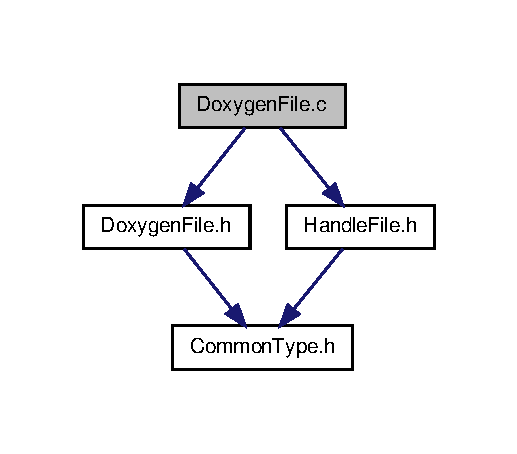
\includegraphics[width=248pt]{DoxygenFile_8c__incl}
\end{center}
\end{figure}
\subsection*{Functions}
\begin{DoxyCompactItemize}
\item 
int \hyperlink{DoxygenFile_8c_a2ef092284bdeff91a581b35199e25e78}{Handle\-Data} (\hyperlink{CommonType_8h_a36cb3b01d81ffd844bbbfb54003e06ec}{U\-I\-N\-T} file\-Name\-Len, \hyperlink{CommonType_8h_a4ae1dab0fb4b072a66584546209e7d58}{B\-Y\-T\-E} $\ast$file\-Name, \hyperlink{CommonType_8h_a4ae1dab0fb4b072a66584546209e7d58}{B\-Y\-T\-E} $\ast$file\-Data)
\end{DoxyCompactItemize}


\subsection{Function Documentation}
\hypertarget{DoxygenFile_8c_a2ef092284bdeff91a581b35199e25e78}{\index{Doxygen\-File.\-c@{Doxygen\-File.\-c}!Handle\-Data@{Handle\-Data}}
\index{Handle\-Data@{Handle\-Data}!DoxygenFile.c@{Doxygen\-File.\-c}}
\subsubsection[{Handle\-Data}]{\setlength{\rightskip}{0pt plus 5cm}int Handle\-Data (
\begin{DoxyParamCaption}
\item[{{\bf U\-I\-N\-T}}]{file\-Name\-Len, }
\item[{{\bf B\-Y\-T\-E} $\ast$}]{file\-Name, }
\item[{{\bf B\-Y\-T\-E} $\ast$}]{file\-Data}
\end{DoxyParamCaption}
)}}\label{DoxygenFile_8c_a2ef092284bdeff91a581b35199e25e78}
写入一些内容 
\begin{DoxyParams}[1]{Parameters}
\mbox{\tt in}  & {\em file\-Name\-Len} & 文件名长度 \\
\hline
\mbox{\tt in}  & {\em file\-Name} & 文件名 \\
\hline
\mbox{\tt out}  & {\em file\-Data} & 文件数据 \\
\hline
\end{DoxyParams}
\begin{DoxyReturn}{Returns}
0,执行成功,非0,失败,详见 \hyperlink{RetCode_8h}{Ret\-Code.\-h} 
\end{DoxyReturn}


References N\-U\-L\-L, and Read\-File().



Referenced by main().



Here is the call graph for this function\-:\nopagebreak
\begin{figure}[H]
\begin{center}
\leavevmode
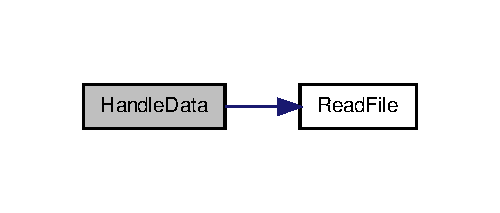
\includegraphics[width=240pt]{DoxygenFile_8c_a2ef092284bdeff91a581b35199e25e78_cgraph}
\end{center}
\end{figure}




Here is the caller graph for this function\-:\nopagebreak
\begin{figure}[H]
\begin{center}
\leavevmode
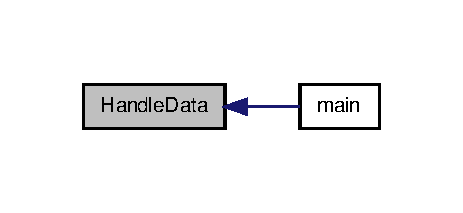
\includegraphics[width=222pt]{DoxygenFile_8c_a2ef092284bdeff91a581b35199e25e78_icgraph}
\end{center}
\end{figure}



\hypertarget{DoxygenFile_8h}{\section{Doxygen\-File.\-h File Reference}
\label{DoxygenFile_8h}\index{Doxygen\-File.\-h@{Doxygen\-File.\-h}}
}


中间层,用于处理数据  


{\ttfamily \#include \char`\"{}Common\-Type.\-h\char`\"{}}\\*
Include dependency graph for Doxygen\-File.\-h\-:\nopagebreak
\begin{figure}[H]
\begin{center}
\leavevmode
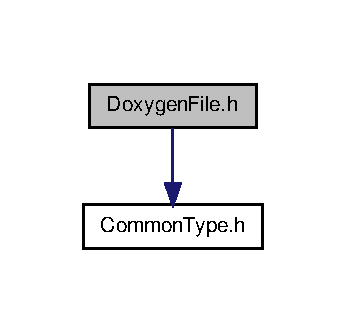
\includegraphics[width=166pt]{DoxygenFile_8h__incl}
\end{center}
\end{figure}
This graph shows which files directly or indirectly include this file\-:\nopagebreak
\begin{figure}[H]
\begin{center}
\leavevmode
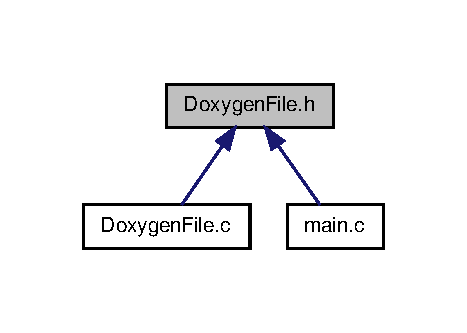
\includegraphics[width=224pt]{DoxygenFile_8h__dep__incl}
\end{center}
\end{figure}
\subsection*{Functions}
\begin{DoxyCompactItemize}
\item 
int \hyperlink{DoxygenFile_8h_a2ef092284bdeff91a581b35199e25e78}{Handle\-Data} (\hyperlink{CommonType_8h_a36cb3b01d81ffd844bbbfb54003e06ec}{U\-I\-N\-T} file\-Name\-Len, \hyperlink{CommonType_8h_a4ae1dab0fb4b072a66584546209e7d58}{B\-Y\-T\-E} $\ast$file\-Name, \hyperlink{CommonType_8h_a4ae1dab0fb4b072a66584546209e7d58}{B\-Y\-T\-E} $\ast$file\-Data)
\end{DoxyCompactItemize}


\subsection{Detailed Description}
中间层,用于处理数据 \begin{DoxyAuthor}{Author}
Vincent 
\end{DoxyAuthor}
\begin{DoxyDate}{Date}
2015-\/5-\/24 
\end{DoxyDate}
\begin{DoxyVersion}{Version}
A001 
\end{DoxyVersion}
\begin{DoxyParagraph}{Copyright (c)\-: Vincent }

\end{DoxyParagraph}


\subsection{Function Documentation}
\hypertarget{DoxygenFile_8h_a2ef092284bdeff91a581b35199e25e78}{\index{Doxygen\-File.\-h@{Doxygen\-File.\-h}!Handle\-Data@{Handle\-Data}}
\index{Handle\-Data@{Handle\-Data}!DoxygenFile.h@{Doxygen\-File.\-h}}
\subsubsection[{Handle\-Data}]{\setlength{\rightskip}{0pt plus 5cm}int Handle\-Data (
\begin{DoxyParamCaption}
\item[{{\bf U\-I\-N\-T}}]{file\-Name\-Len, }
\item[{{\bf B\-Y\-T\-E} $\ast$}]{file\-Name, }
\item[{{\bf B\-Y\-T\-E} $\ast$}]{file\-Data}
\end{DoxyParamCaption}
)}}\label{DoxygenFile_8h_a2ef092284bdeff91a581b35199e25e78}
写入一些内容 
\begin{DoxyParams}[1]{Parameters}
\mbox{\tt in}  & {\em file\-Name\-Len} & 文件名长度 \\
\hline
\mbox{\tt in}  & {\em file\-Name} & 文件名 \\
\hline
\mbox{\tt out}  & {\em file\-Data} & 文件数据 \\
\hline
\end{DoxyParams}
\begin{DoxyReturn}{Returns}
0,执行成功,非0,失败,详见 \hyperlink{RetCode_8h}{Ret\-Code.\-h} 
\end{DoxyReturn}


References N\-U\-L\-L, and Read\-File().



Referenced by main().



Here is the call graph for this function\-:\nopagebreak
\begin{figure}[H]
\begin{center}
\leavevmode
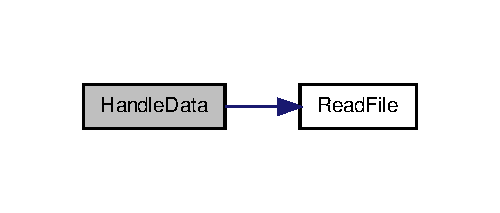
\includegraphics[width=240pt]{DoxygenFile_8h_a2ef092284bdeff91a581b35199e25e78_cgraph}
\end{center}
\end{figure}




Here is the caller graph for this function\-:\nopagebreak
\begin{figure}[H]
\begin{center}
\leavevmode
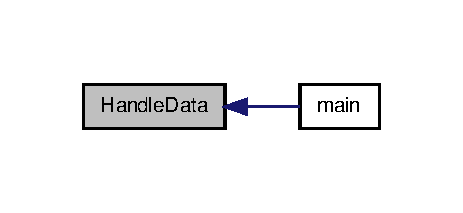
\includegraphics[width=222pt]{DoxygenFile_8h_a2ef092284bdeff91a581b35199e25e78_icgraph}
\end{center}
\end{figure}



\hypertarget{HandleFile_8c}{\section{Handle\-File.\-c File Reference}
\label{HandleFile_8c}\index{Handle\-File.\-c@{Handle\-File.\-c}}
}
{\ttfamily \#include \char`\"{}Handle\-File.\-h\char`\"{}}\\*
{\ttfamily \#include \char`\"{}Ret\-Code.\-h\char`\"{}}\\*
{\ttfamily \#include \char`\"{}Addr\-Define.\-h\char`\"{}}\\*
Include dependency graph for Handle\-File.\-c\-:\nopagebreak
\begin{figure}[H]
\begin{center}
\leavevmode
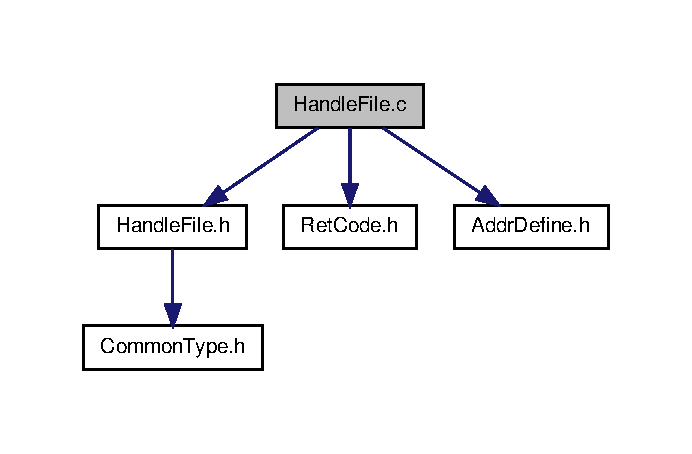
\includegraphics[width=332pt]{HandleFile_8c__incl}
\end{center}
\end{figure}
\subsection*{Functions}
\begin{DoxyCompactItemize}
\item 
\hyperlink{CommonType_8h_a36cb3b01d81ffd844bbbfb54003e06ec}{U\-I\-N\-T} \hyperlink{HandleFile_8c_a8741717ea9029d93b7addf8158ebad0c}{Read\-File} (\hyperlink{CommonType_8h_a36cb3b01d81ffd844bbbfb54003e06ec}{U\-I\-N\-T} file\-Name\-Len, \hyperlink{CommonType_8h_a4ae1dab0fb4b072a66584546209e7d58}{B\-Y\-T\-E} $\ast$file\-Name, \hyperlink{CommonType_8h_a36cb3b01d81ffd844bbbfb54003e06ec}{U\-I\-N\-T} data\-Len, \hyperlink{CommonType_8h_a4ae1dab0fb4b072a66584546209e7d58}{B\-Y\-T\-E} $\ast$file\-Data)
\begin{DoxyCompactList}\small\item\em 操作文件 \end{DoxyCompactList}\item 
\hyperlink{CommonType_8h_a36cb3b01d81ffd844bbbfb54003e06ec}{U\-I\-N\-T} \hyperlink{HandleFile_8c_afede9fe93381c9a702a420e90eb553a6}{Write\-File} (\hyperlink{CommonType_8h_a36cb3b01d81ffd844bbbfb54003e06ec}{U\-I\-N\-T} file\-Name\-Len, \hyperlink{CommonType_8h_a4ae1dab0fb4b072a66584546209e7d58}{B\-Y\-T\-E} $\ast$file\-Name, \hyperlink{CommonType_8h_a4ae1dab0fb4b072a66584546209e7d58}{B\-Y\-T\-E} $\ast$file\-Data)
\item 
\hyperlink{CommonType_8h_a36cb3b01d81ffd844bbbfb54003e06ec}{U\-I\-N\-T} \hyperlink{HandleFile_8c_a8b6ef3269dda1e36066846707cc4166e}{Erase\-File} (\hyperlink{CommonType_8h_a36cb3b01d81ffd844bbbfb54003e06ec}{U\-I\-N\-T} file\-Name\-Len, \hyperlink{CommonType_8h_a4ae1dab0fb4b072a66584546209e7d58}{B\-Y\-T\-E} $\ast$file\-Name)
\end{DoxyCompactItemize}


\subsection{Function Documentation}
\hypertarget{HandleFile_8c_a8b6ef3269dda1e36066846707cc4166e}{\index{Handle\-File.\-c@{Handle\-File.\-c}!Erase\-File@{Erase\-File}}
\index{Erase\-File@{Erase\-File}!HandleFile.c@{Handle\-File.\-c}}
\subsubsection[{Erase\-File}]{\setlength{\rightskip}{0pt plus 5cm}{\bf U\-I\-N\-T} Erase\-File (
\begin{DoxyParamCaption}
\item[{{\bf U\-I\-N\-T}}]{file\-Name\-Len, }
\item[{{\bf B\-Y\-T\-E} $\ast$}]{file\-Name}
\end{DoxyParamCaption}
)}}\label{HandleFile_8c_a8b6ef3269dda1e36066846707cc4166e}
擦除文件 
\begin{DoxyParams}[1]{Parameters}
\mbox{\tt in}  & {\em file\-Name\-Len} & 文件名长度 \\
\hline
\mbox{\tt in}  & {\em file\-Name} & 文件名 \\
\hline
\end{DoxyParams}
\begin{DoxyReturn}{Returns}
0,执行成功,非0,失败,详见 \hyperlink{RetCode_8h}{Ret\-Code.\-h} 
\end{DoxyReturn}
\begin{DoxySeeAlso}{See Also}

\end{DoxySeeAlso}
\begin{DoxyNote}{Note}

\end{DoxyNote}


References S\-U\-C\-C\-E\-S\-S.

\hypertarget{HandleFile_8c_a8741717ea9029d93b7addf8158ebad0c}{\index{Handle\-File.\-c@{Handle\-File.\-c}!Read\-File@{Read\-File}}
\index{Read\-File@{Read\-File}!HandleFile.c@{Handle\-File.\-c}}
\subsubsection[{Read\-File}]{\setlength{\rightskip}{0pt plus 5cm}{\bf U\-I\-N\-T} Read\-File (
\begin{DoxyParamCaption}
\item[{{\bf U\-I\-N\-T}}]{file\-Name\-Len, }
\item[{{\bf B\-Y\-T\-E} $\ast$}]{file\-Name, }
\item[{{\bf U\-I\-N\-T}}]{data\-Len, }
\item[{{\bf B\-Y\-T\-E} $\ast$}]{file\-Data}
\end{DoxyParamCaption}
)}}\label{HandleFile_8c_a8741717ea9029d93b7addf8158ebad0c}


操作文件 

读取文件 
\begin{DoxyParams}[1]{Parameters}
\mbox{\tt in}  & {\em file\-Name\-Len} & 文件名长度 \\
\hline
\mbox{\tt in}  & {\em file\-Name} & 文件名 \\
\hline
\mbox{\tt in}  & {\em data\-Len} & 数据长度 \\
\hline
\mbox{\tt out}  & {\em file\-Data} & 输出数据 \\
\hline
\end{DoxyParams}
\begin{DoxyReturn}{Returns}
0,执行成功,非0,失败,详见 \hyperlink{RetCode_8h}{Ret\-Code.\-h} 
\end{DoxyReturn}
\begin{DoxySeeAlso}{See Also}

\end{DoxySeeAlso}
\begin{DoxyNote}{Note}

\end{DoxyNote}


References S\-U\-C\-C\-E\-S\-S.



Referenced by Handle\-Data().



Here is the caller graph for this function\-:\nopagebreak
\begin{figure}[H]
\begin{center}
\leavevmode
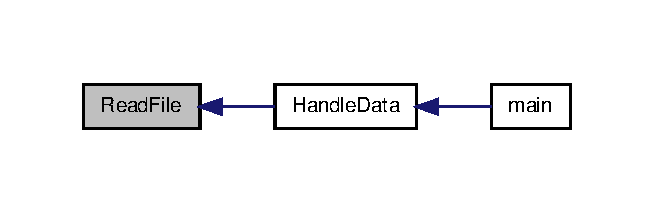
\includegraphics[width=314pt]{HandleFile_8c_a8741717ea9029d93b7addf8158ebad0c_icgraph}
\end{center}
\end{figure}


\hypertarget{HandleFile_8c_afede9fe93381c9a702a420e90eb553a6}{\index{Handle\-File.\-c@{Handle\-File.\-c}!Write\-File@{Write\-File}}
\index{Write\-File@{Write\-File}!HandleFile.c@{Handle\-File.\-c}}
\subsubsection[{Write\-File}]{\setlength{\rightskip}{0pt plus 5cm}{\bf U\-I\-N\-T} Write\-File (
\begin{DoxyParamCaption}
\item[{{\bf U\-I\-N\-T}}]{file\-Name\-Len, }
\item[{{\bf B\-Y\-T\-E} $\ast$}]{file\-Name, }
\item[{{\bf B\-Y\-T\-E} $\ast$}]{file\-Data}
\end{DoxyParamCaption}
)}}\label{HandleFile_8c_afede9fe93381c9a702a420e90eb553a6}
写入文件 
\begin{DoxyParams}[1]{Parameters}
\mbox{\tt in}  & {\em file\-Name\-Len} & 文件名长度 \\
\hline
\mbox{\tt in}  & {\em file\-Name} & 文件名 \\
\hline
\mbox{\tt out}  & {\em file\-Data} & 输出数据 \\
\hline
\end{DoxyParams}
\begin{DoxyReturn}{Returns}
0,执行成功,非0,失败,详见 \hyperlink{RetCode_8h}{Ret\-Code.\-h} 
\end{DoxyReturn}
\begin{DoxySeeAlso}{See Also}

\end{DoxySeeAlso}
\begin{DoxyNote}{Note}

\end{DoxyNote}


References S\-U\-C\-C\-E\-S\-S.


\hypertarget{HandleFile_8h}{\section{Handle\-File.\-h File Reference}
\label{HandleFile_8h}\index{Handle\-File.\-h@{Handle\-File.\-h}}
}
{\ttfamily \#include \char`\"{}Common\-Type.\-h\char`\"{}}\\*
Include dependency graph for Handle\-File.\-h\-:\nopagebreak
\begin{figure}[H]
\begin{center}
\leavevmode
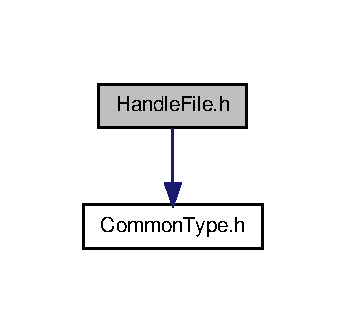
\includegraphics[width=166pt]{HandleFile_8h__incl}
\end{center}
\end{figure}
This graph shows which files directly or indirectly include this file\-:\nopagebreak
\begin{figure}[H]
\begin{center}
\leavevmode
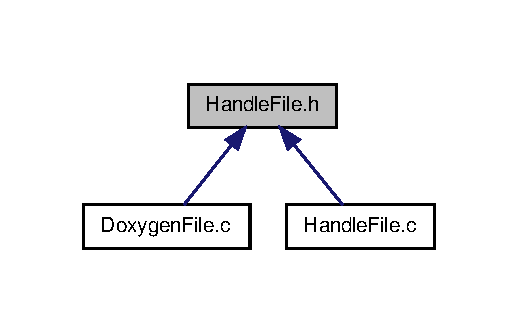
\includegraphics[width=248pt]{HandleFile_8h__dep__incl}
\end{center}
\end{figure}
\subsection*{Functions}
\begin{DoxyCompactItemize}
\item 
\hyperlink{CommonType_8h_a36cb3b01d81ffd844bbbfb54003e06ec}{U\-I\-N\-T} \hyperlink{HandleFile_8h_a8741717ea9029d93b7addf8158ebad0c}{Read\-File} (\hyperlink{CommonType_8h_a36cb3b01d81ffd844bbbfb54003e06ec}{U\-I\-N\-T} file\-Name\-Len, \hyperlink{CommonType_8h_a4ae1dab0fb4b072a66584546209e7d58}{B\-Y\-T\-E} $\ast$file\-Name, \hyperlink{CommonType_8h_a36cb3b01d81ffd844bbbfb54003e06ec}{U\-I\-N\-T} data\-Len, \hyperlink{CommonType_8h_a4ae1dab0fb4b072a66584546209e7d58}{B\-Y\-T\-E} $\ast$file\-Data)
\begin{DoxyCompactList}\small\item\em 操作文件 \end{DoxyCompactList}\item 
\hyperlink{CommonType_8h_a36cb3b01d81ffd844bbbfb54003e06ec}{U\-I\-N\-T} \hyperlink{HandleFile_8h_afede9fe93381c9a702a420e90eb553a6}{Write\-File} (\hyperlink{CommonType_8h_a36cb3b01d81ffd844bbbfb54003e06ec}{U\-I\-N\-T} file\-Name\-Len, \hyperlink{CommonType_8h_a4ae1dab0fb4b072a66584546209e7d58}{B\-Y\-T\-E} $\ast$file\-Name, \hyperlink{CommonType_8h_a4ae1dab0fb4b072a66584546209e7d58}{B\-Y\-T\-E} $\ast$file\-Data)
\item 
\hyperlink{CommonType_8h_a36cb3b01d81ffd844bbbfb54003e06ec}{U\-I\-N\-T} \hyperlink{HandleFile_8h_a8b6ef3269dda1e36066846707cc4166e}{Erase\-File} (\hyperlink{CommonType_8h_a36cb3b01d81ffd844bbbfb54003e06ec}{U\-I\-N\-T} file\-Name\-Len, \hyperlink{CommonType_8h_a4ae1dab0fb4b072a66584546209e7d58}{B\-Y\-T\-E} $\ast$file\-Name)
\end{DoxyCompactItemize}


\subsection{Function Documentation}
\hypertarget{HandleFile_8h_a8b6ef3269dda1e36066846707cc4166e}{\index{Handle\-File.\-h@{Handle\-File.\-h}!Erase\-File@{Erase\-File}}
\index{Erase\-File@{Erase\-File}!HandleFile.h@{Handle\-File.\-h}}
\subsubsection[{Erase\-File}]{\setlength{\rightskip}{0pt plus 5cm}{\bf U\-I\-N\-T} Erase\-File (
\begin{DoxyParamCaption}
\item[{{\bf U\-I\-N\-T}}]{file\-Name\-Len, }
\item[{{\bf B\-Y\-T\-E} $\ast$}]{file\-Name}
\end{DoxyParamCaption}
)}}\label{HandleFile_8h_a8b6ef3269dda1e36066846707cc4166e}
擦除文件 
\begin{DoxyParams}[1]{Parameters}
\mbox{\tt in}  & {\em file\-Name\-Len} & 文件名长度 \\
\hline
\mbox{\tt in}  & {\em file\-Name} & 文件名 \\
\hline
\end{DoxyParams}
\begin{DoxyReturn}{Returns}
0,执行成功,非0,失败,详见 \hyperlink{RetCode_8h}{Ret\-Code.\-h} 
\end{DoxyReturn}
\begin{DoxySeeAlso}{See Also}

\end{DoxySeeAlso}
\begin{DoxyNote}{Note}

\end{DoxyNote}


References S\-U\-C\-C\-E\-S\-S.

\hypertarget{HandleFile_8h_a8741717ea9029d93b7addf8158ebad0c}{\index{Handle\-File.\-h@{Handle\-File.\-h}!Read\-File@{Read\-File}}
\index{Read\-File@{Read\-File}!HandleFile.h@{Handle\-File.\-h}}
\subsubsection[{Read\-File}]{\setlength{\rightskip}{0pt plus 5cm}{\bf U\-I\-N\-T} Read\-File (
\begin{DoxyParamCaption}
\item[{{\bf U\-I\-N\-T}}]{file\-Name\-Len, }
\item[{{\bf B\-Y\-T\-E} $\ast$}]{file\-Name, }
\item[{{\bf U\-I\-N\-T}}]{data\-Len, }
\item[{{\bf B\-Y\-T\-E} $\ast$}]{file\-Data}
\end{DoxyParamCaption}
)}}\label{HandleFile_8h_a8741717ea9029d93b7addf8158ebad0c}


操作文件 

le \hyperlink{HandleFile_8h}{Handle\-File.\-h}

所有涉及文件操作 \begin{DoxyAuthor}{Author}
Vincent 
\end{DoxyAuthor}
\begin{DoxyDate}{Date}
2015-\/5-\/24 
\end{DoxyDate}
\begin{DoxyVersion}{Version}
A001 
\end{DoxyVersion}
\begin{DoxyParagraph}{Copyright (c)\-: Vincent }

\end{DoxyParagraph}
读取文件 
\begin{DoxyParams}[1]{Parameters}
\mbox{\tt in}  & {\em file\-Name\-Len} & 文件名长度 \\
\hline
\mbox{\tt in}  & {\em file\-Name} & 文件名 \\
\hline
\mbox{\tt in}  & {\em data\-Len} & 数据长度 \\
\hline
\mbox{\tt out}  & {\em file\-Data} & 输出数据 \\
\hline
\end{DoxyParams}
\begin{DoxyReturn}{Returns}
0,执行成功,非0,失败,详见 \hyperlink{RetCode_8h}{Ret\-Code.\-h} 
\end{DoxyReturn}
\begin{DoxySeeAlso}{See Also}

\end{DoxySeeAlso}
\begin{DoxyNote}{Note}

\end{DoxyNote}


References S\-U\-C\-C\-E\-S\-S.



Referenced by Handle\-Data().



Here is the caller graph for this function\-:\nopagebreak
\begin{figure}[H]
\begin{center}
\leavevmode
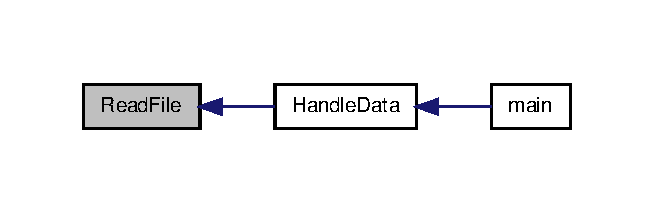
\includegraphics[width=314pt]{HandleFile_8h_a8741717ea9029d93b7addf8158ebad0c_icgraph}
\end{center}
\end{figure}


\hypertarget{HandleFile_8h_afede9fe93381c9a702a420e90eb553a6}{\index{Handle\-File.\-h@{Handle\-File.\-h}!Write\-File@{Write\-File}}
\index{Write\-File@{Write\-File}!HandleFile.h@{Handle\-File.\-h}}
\subsubsection[{Write\-File}]{\setlength{\rightskip}{0pt plus 5cm}{\bf U\-I\-N\-T} Write\-File (
\begin{DoxyParamCaption}
\item[{{\bf U\-I\-N\-T}}]{file\-Name\-Len, }
\item[{{\bf B\-Y\-T\-E} $\ast$}]{file\-Name, }
\item[{{\bf B\-Y\-T\-E} $\ast$}]{file\-Data}
\end{DoxyParamCaption}
)}}\label{HandleFile_8h_afede9fe93381c9a702a420e90eb553a6}
写入文件 
\begin{DoxyParams}[1]{Parameters}
\mbox{\tt in}  & {\em file\-Name\-Len} & 文件名长度 \\
\hline
\mbox{\tt in}  & {\em file\-Name} & 文件名 \\
\hline
\mbox{\tt out}  & {\em file\-Data} & 输出数据 \\
\hline
\end{DoxyParams}
\begin{DoxyReturn}{Returns}
0,执行成功,非0,失败,详见 \hyperlink{RetCode_8h}{Ret\-Code.\-h} 
\end{DoxyReturn}
\begin{DoxySeeAlso}{See Also}

\end{DoxySeeAlso}
\begin{DoxyNote}{Note}

\end{DoxyNote}


References S\-U\-C\-C\-E\-S\-S.


\hypertarget{main_8c}{\section{main.\-c File Reference}
\label{main_8c}\index{main.\-c@{main.\-c}}
}
{\ttfamily \#include \char`\"{}Doxygen\-File.\-h\char`\"{}}\\*
{\ttfamily \#include \char`\"{}Common\-Type.\-h\char`\"{}}\\*
Include dependency graph for main.\-c\-:\nopagebreak
\begin{figure}[H]
\begin{center}
\leavevmode
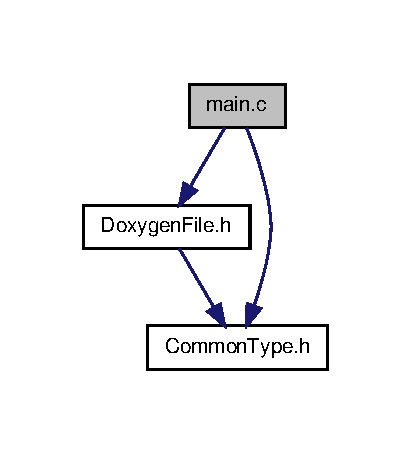
\includegraphics[width=197pt]{main_8c__incl}
\end{center}
\end{figure}
\subsection*{Functions}
\begin{DoxyCompactItemize}
\item 
void \hyperlink{main_8c_acdef7a1fd863a6d3770c1268cb06add3}{main} ()
\end{DoxyCompactItemize}


\subsection{Function Documentation}
\hypertarget{main_8c_acdef7a1fd863a6d3770c1268cb06add3}{\index{main.\-c@{main.\-c}!main@{main}}
\index{main@{main}!main.c@{main.\-c}}
\subsubsection[{main}]{\setlength{\rightskip}{0pt plus 5cm}void main (
\begin{DoxyParamCaption}
{}
\end{DoxyParamCaption}
)}}\label{main_8c_acdef7a1fd863a6d3770c1268cb06add3}


References Handle\-Data(), and N\-U\-L\-L.



Here is the call graph for this function\-:\nopagebreak
\begin{figure}[H]
\begin{center}
\leavevmode
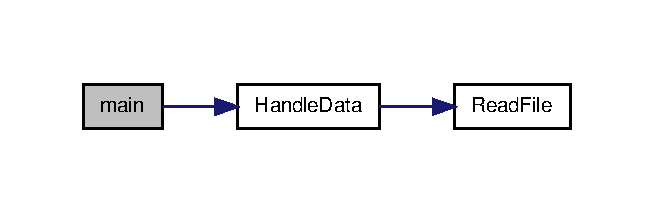
\includegraphics[width=314pt]{main_8c_acdef7a1fd863a6d3770c1268cb06add3_cgraph}
\end{center}
\end{figure}



\hypertarget{RetCode_8h}{\section{Ret\-Code.\-h File Reference}
\label{RetCode_8h}\index{Ret\-Code.\-h@{Ret\-Code.\-h}}
}


错误码返回值  


This graph shows which files directly or indirectly include this file\-:\nopagebreak
\begin{figure}[H]
\begin{center}
\leavevmode
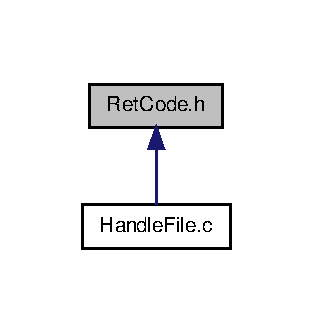
\includegraphics[width=150pt]{RetCode_8h__dep__incl}
\end{center}
\end{figure}
\subsection*{Macros}
\begin{Indent}{\bf 执行状态}\par
\begin{DoxyCompactItemize}
\item 
\#define \hyperlink{RetCode_8h_aa90cac659d18e8ef6294c7ae337f6b58}{S\-U\-C\-C\-E\-S\-S}~0x00000000
\begin{DoxyCompactList}\small\item\em 执行成功 \end{DoxyCompactList}\item 
\#define \hyperlink{RetCode_8h_ac839a0b40c756c94bffbfe49eeea544e}{E\-R\-R\-\_\-\-P\-A\-R\-A\-\_\-\-L\-E\-N}~0x00000001
\begin{DoxyCompactList}\small\item\em 长度错误 \end{DoxyCompactList}\item 
\#define \hyperlink{RetCode_8h_ad155c5be2130bc4bff24dc31096fe605}{E\-R\-R\-\_\-\-N\-U\-L\-L\-\_\-\-P\-O\-I\-N\-T}~0x00000002
\begin{DoxyCompactList}\small\item\em 空指针错误 \end{DoxyCompactList}\item 
\#define \hyperlink{RetCode_8h_ad822bcd976fd01d6c1d126994b24d9f2}{E\-R\-R\-\_\-\-P\-A\-R\-A\-\_\-\-T\-Y\-P\-E}~0x00000003
\begin{DoxyCompactList}\small\item\em 参数类型错误 \end{DoxyCompactList}\end{DoxyCompactItemize}
\end{Indent}


\subsection{Detailed Description}
错误码返回值 \begin{DoxyAuthor}{Author}
Vincent 
\end{DoxyAuthor}
\begin{DoxyDate}{Date}
2015-\/5-\/24 
\end{DoxyDate}
\begin{DoxyVersion}{Version}
A001 
\end{DoxyVersion}
\begin{DoxyParagraph}{Copyright (c)\-: Vincent }

\end{DoxyParagraph}


\subsection{Macro Definition Documentation}
\hypertarget{RetCode_8h_ad155c5be2130bc4bff24dc31096fe605}{\index{Ret\-Code.\-h@{Ret\-Code.\-h}!E\-R\-R\-\_\-\-N\-U\-L\-L\-\_\-\-P\-O\-I\-N\-T@{E\-R\-R\-\_\-\-N\-U\-L\-L\-\_\-\-P\-O\-I\-N\-T}}
\index{E\-R\-R\-\_\-\-N\-U\-L\-L\-\_\-\-P\-O\-I\-N\-T@{E\-R\-R\-\_\-\-N\-U\-L\-L\-\_\-\-P\-O\-I\-N\-T}!RetCode.h@{Ret\-Code.\-h}}
\subsubsection[{E\-R\-R\-\_\-\-N\-U\-L\-L\-\_\-\-P\-O\-I\-N\-T}]{\setlength{\rightskip}{0pt plus 5cm}\#define E\-R\-R\-\_\-\-N\-U\-L\-L\-\_\-\-P\-O\-I\-N\-T~0x00000002}}\label{RetCode_8h_ad155c5be2130bc4bff24dc31096fe605}


空指针错误 

\hypertarget{RetCode_8h_ac839a0b40c756c94bffbfe49eeea544e}{\index{Ret\-Code.\-h@{Ret\-Code.\-h}!E\-R\-R\-\_\-\-P\-A\-R\-A\-\_\-\-L\-E\-N@{E\-R\-R\-\_\-\-P\-A\-R\-A\-\_\-\-L\-E\-N}}
\index{E\-R\-R\-\_\-\-P\-A\-R\-A\-\_\-\-L\-E\-N@{E\-R\-R\-\_\-\-P\-A\-R\-A\-\_\-\-L\-E\-N}!RetCode.h@{Ret\-Code.\-h}}
\subsubsection[{E\-R\-R\-\_\-\-P\-A\-R\-A\-\_\-\-L\-E\-N}]{\setlength{\rightskip}{0pt plus 5cm}\#define E\-R\-R\-\_\-\-P\-A\-R\-A\-\_\-\-L\-E\-N~0x00000001}}\label{RetCode_8h_ac839a0b40c756c94bffbfe49eeea544e}


长度错误 

\hypertarget{RetCode_8h_ad822bcd976fd01d6c1d126994b24d9f2}{\index{Ret\-Code.\-h@{Ret\-Code.\-h}!E\-R\-R\-\_\-\-P\-A\-R\-A\-\_\-\-T\-Y\-P\-E@{E\-R\-R\-\_\-\-P\-A\-R\-A\-\_\-\-T\-Y\-P\-E}}
\index{E\-R\-R\-\_\-\-P\-A\-R\-A\-\_\-\-T\-Y\-P\-E@{E\-R\-R\-\_\-\-P\-A\-R\-A\-\_\-\-T\-Y\-P\-E}!RetCode.h@{Ret\-Code.\-h}}
\subsubsection[{E\-R\-R\-\_\-\-P\-A\-R\-A\-\_\-\-T\-Y\-P\-E}]{\setlength{\rightskip}{0pt plus 5cm}\#define E\-R\-R\-\_\-\-P\-A\-R\-A\-\_\-\-T\-Y\-P\-E~0x00000003}}\label{RetCode_8h_ad822bcd976fd01d6c1d126994b24d9f2}


参数类型错误 

\hypertarget{RetCode_8h_aa90cac659d18e8ef6294c7ae337f6b58}{\index{Ret\-Code.\-h@{Ret\-Code.\-h}!S\-U\-C\-C\-E\-S\-S@{S\-U\-C\-C\-E\-S\-S}}
\index{S\-U\-C\-C\-E\-S\-S@{S\-U\-C\-C\-E\-S\-S}!RetCode.h@{Ret\-Code.\-h}}
\subsubsection[{S\-U\-C\-C\-E\-S\-S}]{\setlength{\rightskip}{0pt plus 5cm}\#define S\-U\-C\-C\-E\-S\-S~0x00000000}}\label{RetCode_8h_aa90cac659d18e8ef6294c7ae337f6b58}


执行成功 



Referenced by Erase\-File(), Read\-File(), and Write\-File().


\addcontentsline{toc}{part}{Index}
\printindex
\end{document}
